\documentclass{article}
\usepackage{amsmath}
\usepackage{amssymb}
\usepackage{geometry}
\usepackage{graphicx}
\usepackage{placeins}

\begin{document}

\section*{\centering Unsuitability of Delaunay graph mapping for generation of curved meshes}	
While Delaunay graph mapping (DGM) is a very efficient scheme for accomplishing many types of mesh movement, it has a characteristic because of which it is unsuitable for certain meshes and motions. This is the fact that the movement of a node depends only on the motion of the Delaunay element containing it, not necessarily on the motion of the nearest boundary facets.

In case of curved mesh generation for highly anisotropic viscous meshes, it is possible for some Delaunay triangulation facets make angles with the boundary that are very different from 90 degrees (see figure \ref{dg}). Then we may have at least two issues.
\begin{itemize}
\item[1.] Interior points close to a boundary facet can be influenced by another boundary facet far away having a very different curvature.
\item[2.] It may be the case that an interior point is not at all influenced by the closest boundary facet.
\end{itemize}
These issues lead to low curved mesh quality in certain regions, and even invalid elements. We could try using DG-RBF (interpolation by radial basis functions in a Delaunay graph) to help alleviate issue (1), but issue (2) would still persist.

Figure \ref{wmesh} shows a viscous mesh of a 3-element airfoil. Figures \ref{dg} and \ref{mesh} show a portion of its slat. Figure \ref{dg} shows the Delaunay graph and figure \ref{mesh} shows the deformed mesh. We can see that the DG lines make an angle very different from 90 degrees with the boundary. It is clear how points originally in a straight line deform in an oscillatory manner because successive points depend on different Delaunay elements, and different Delaunay elements have different movements depending on which boundary nodes they contain.
\FloatBarrier
\begin{figure}[!h]
	\centering
	\includegraphics[scale=0.28]{3-airfoil}
	\caption{Mesh of a 3-element airfoil}
	\label{wmesh}
\end{figure}
\clearpage
\begin{figure}[p!]
	\centering
	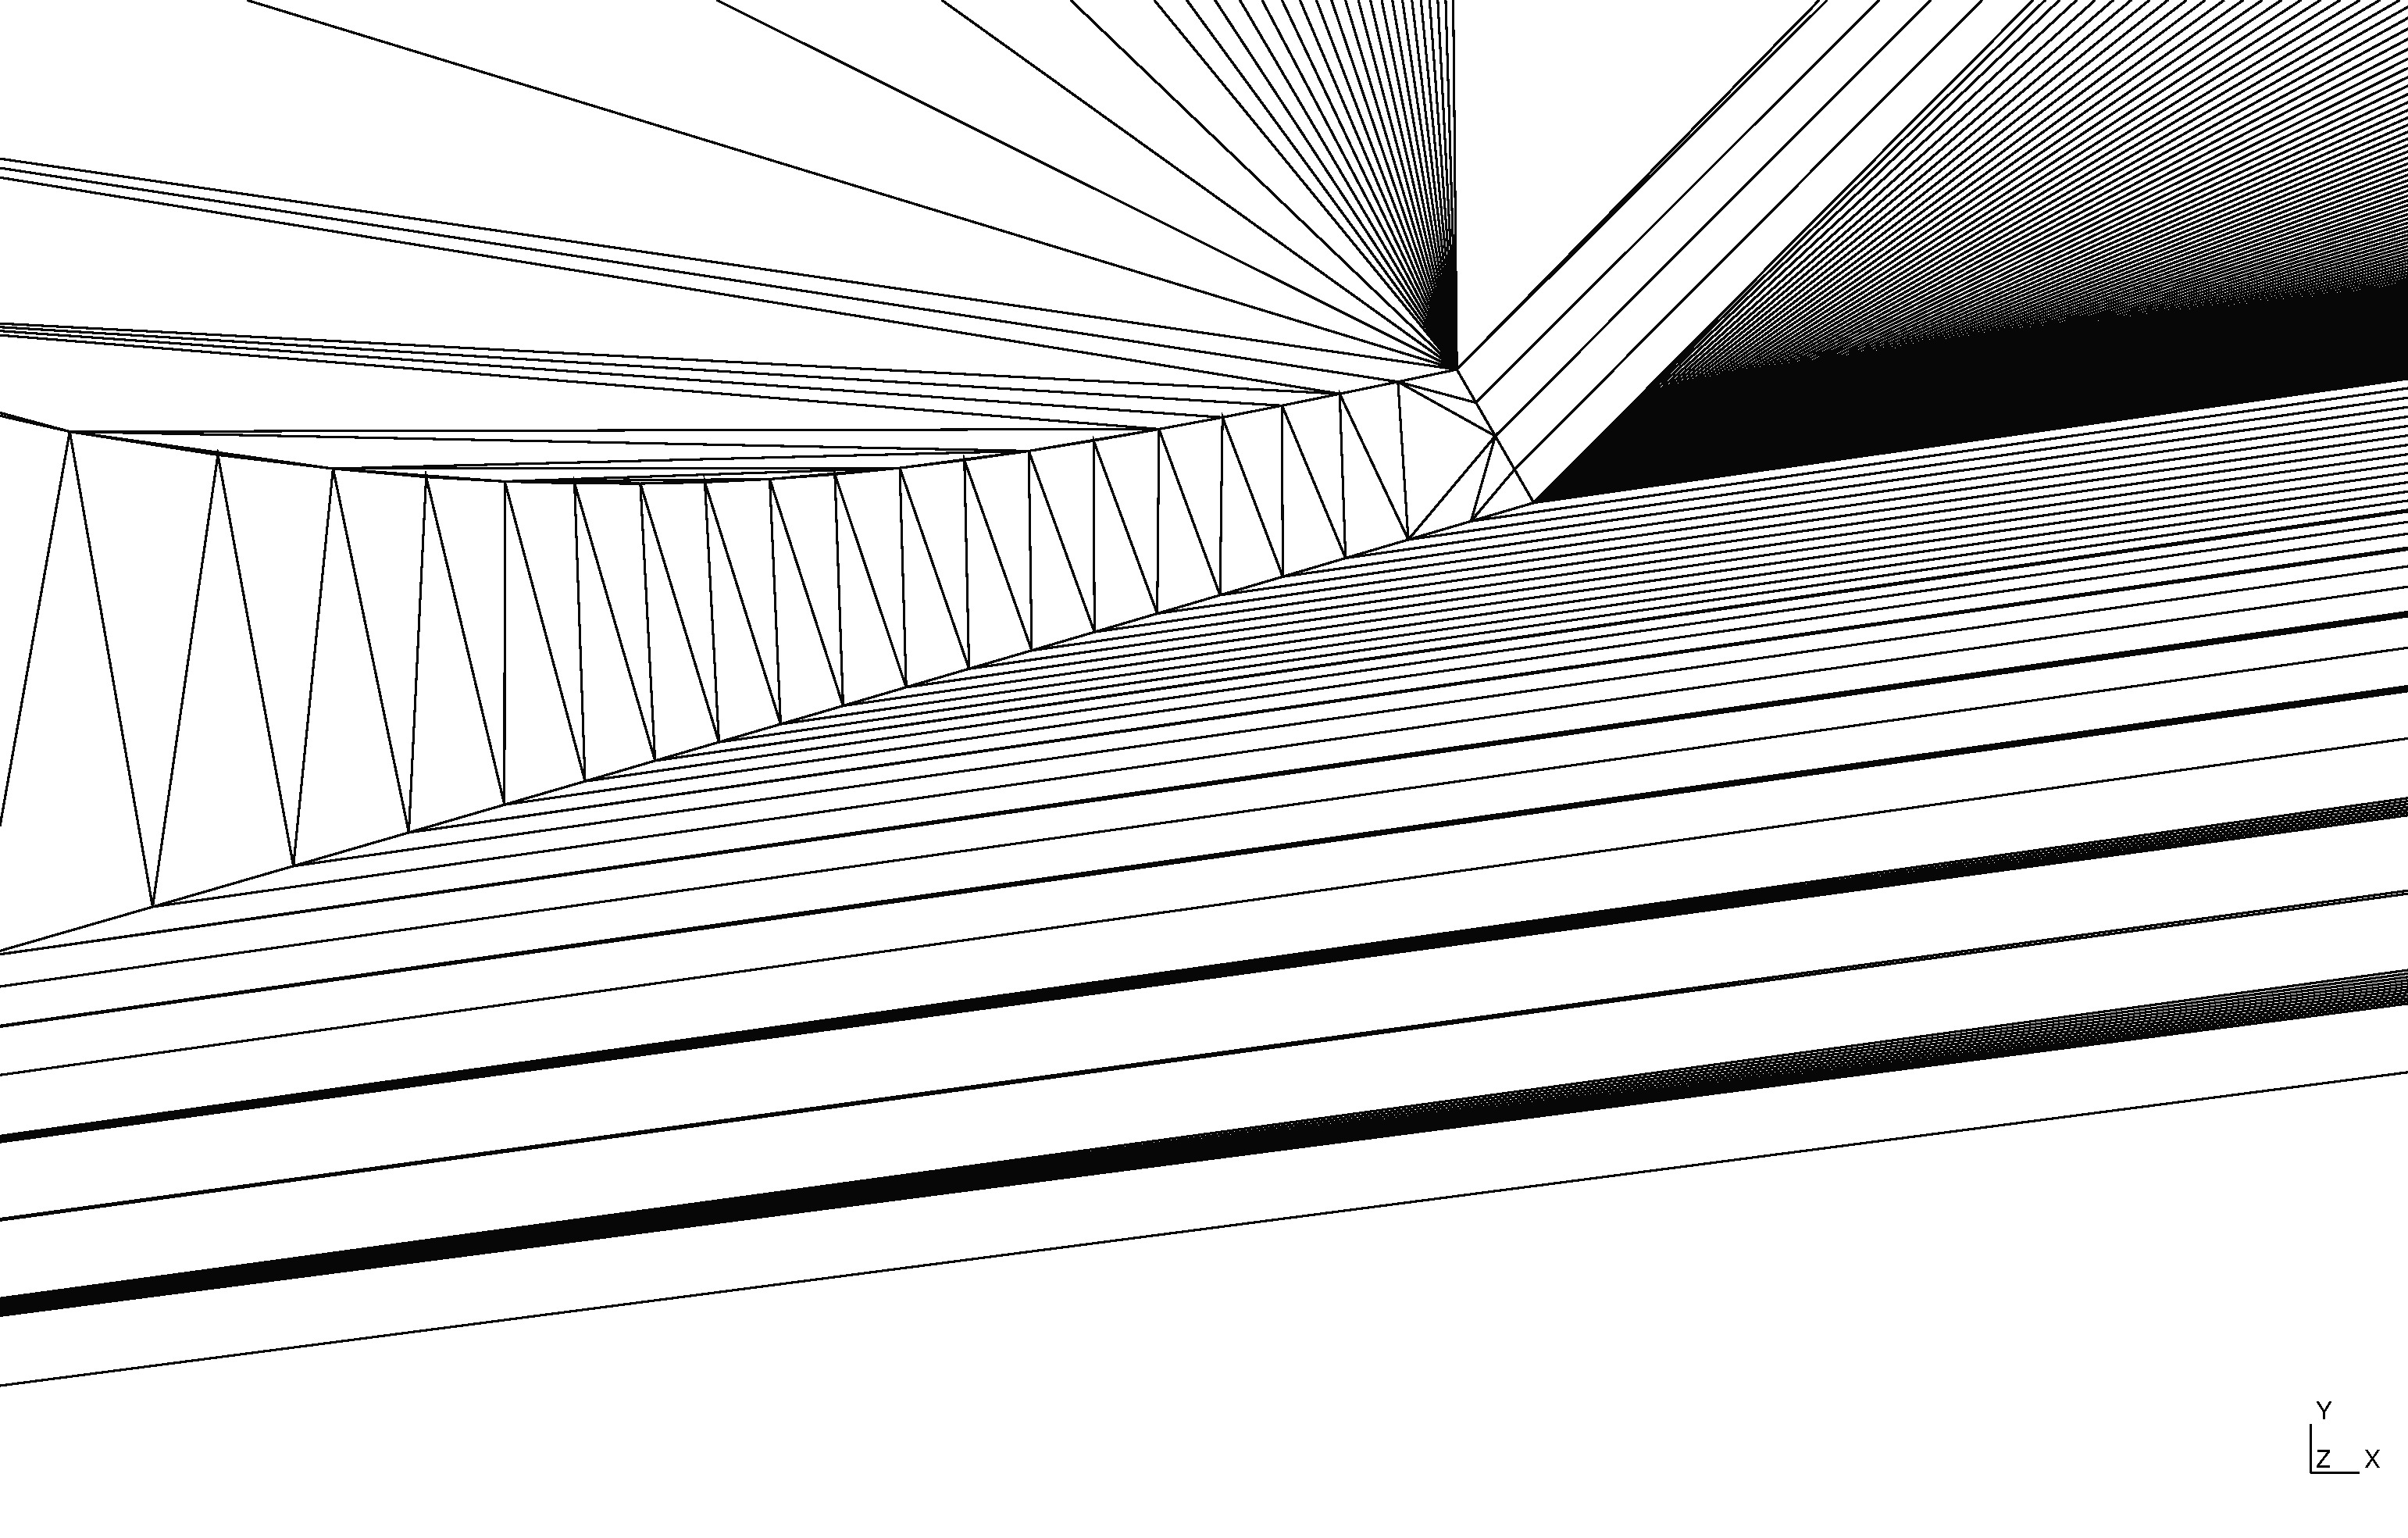
\includegraphics[scale=0.25]{dg-3airfoil-zoomed}
	\caption{Portion of the Delaunay graph near the lower part of the slat}
	\label{dg}
\end{figure}
\begin{figure}[p!]
	\centering
	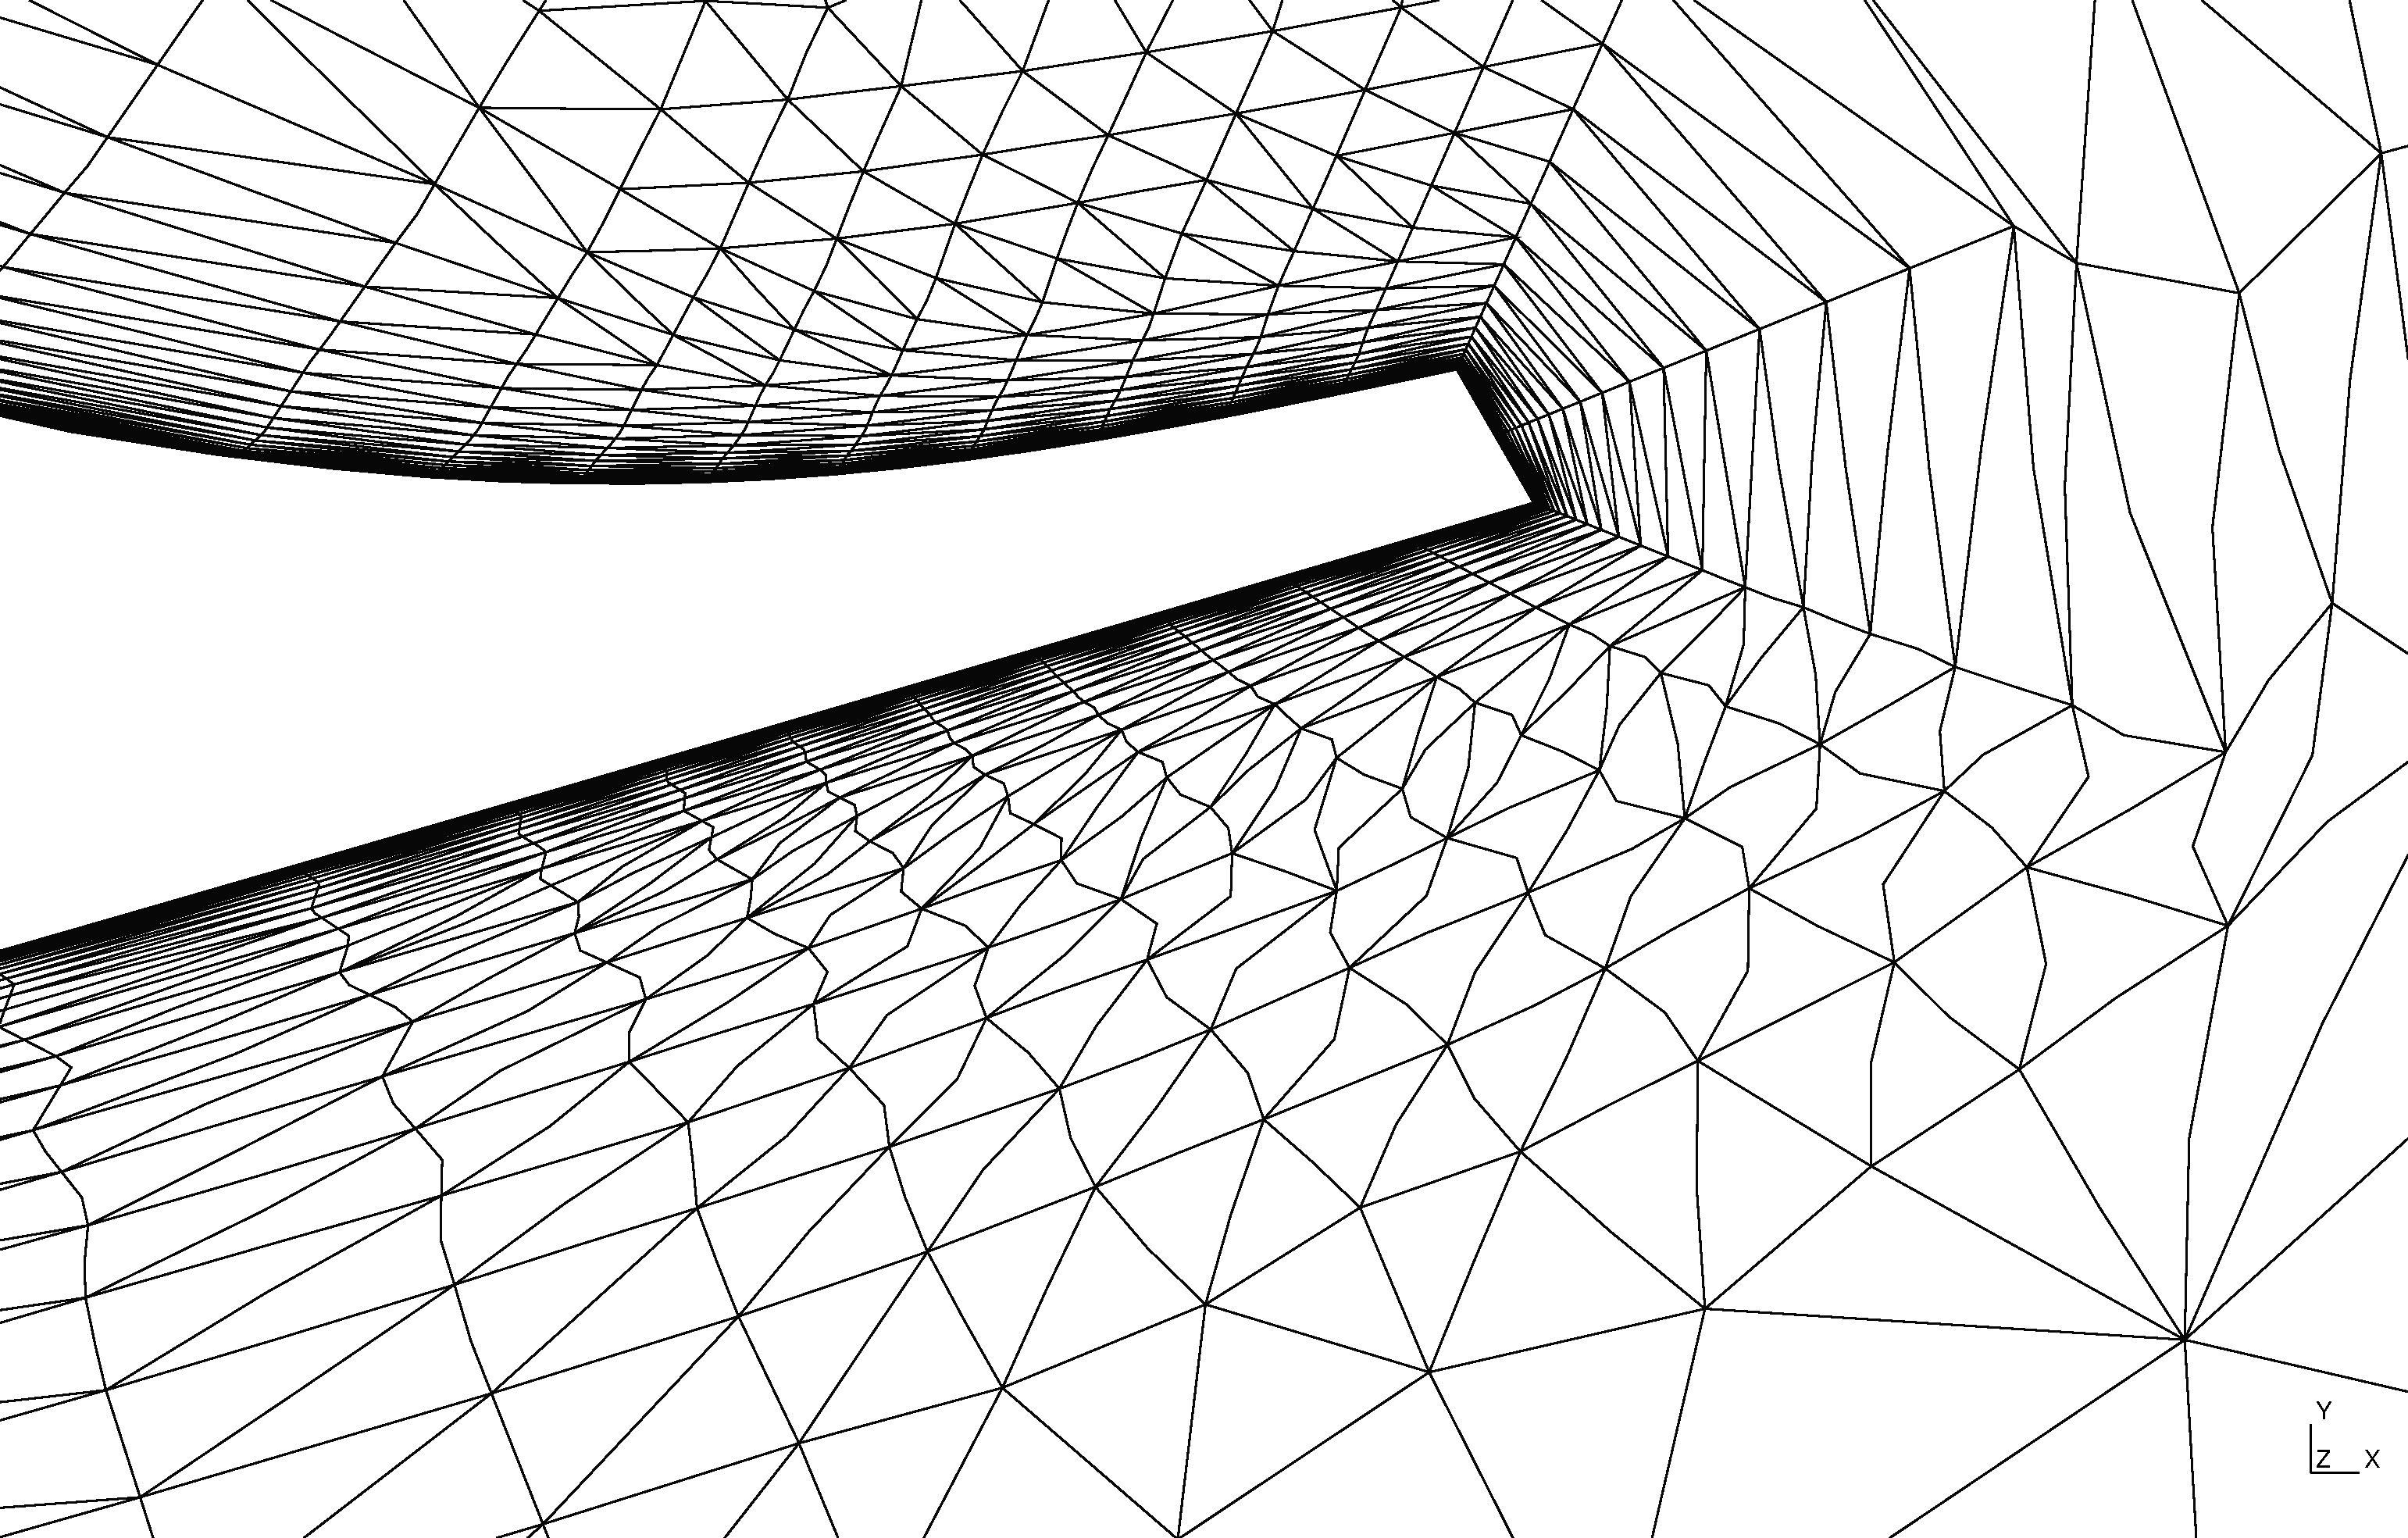
\includegraphics[scale=0.25]{mesh-3airfoil-zoomed}
	\caption{Portion of the mesh near the lower part of the slat}
	\label{mesh}
\end{figure}

\end{document}
